\documentclass[12pt]{article}
\usepackage{amsmath}
\usepackage{amssymb}
\usepackage[margin=2.5cm]{geometry}
\usepackage{physics}
\usepackage[hidelinks]{hyperref}
\usepackage[dvipsnames]{xcolor}
\usepackage[indent=12pt]{parskip}
\usepackage{enumitem}
\usepackage{algorithm}
\usepackage{stmaryrd}
\SetSymbolFont{stmry}{bold}{U}{stmry}{m}{n}

\usepackage{booktabs}
\usepackage{algpseudocode} %[noend]
\usepackage{titling}
\usepackage[
    font=small, skip=6pt, labelfont=bf, labelsep=period, 
    format=hang, margin={5pt, 6pt}
]{caption}
\usepackage{graphicx}
% \usepackage{svg}
    
\usepackage{tikz}
\usetikzlibrary{
  calc, patterns, angles, quotes,
  decorations.pathmorphing, decorations.markings, decorations.text,
  shapes, shapes.multipart,backgrounds,arrows.meta,overlay-beamer-styles,
  external
}
\usepackage{epigraph}

\newcommand{\Sin}{%
  \mathop{\sbox0{$\cos$}\makebox[\wd0][r]{$\sin$}}%
}

\setcounter{tocdepth}{2}
% \setlength{\droptitle}{-3em}
\setlist[itemize]{label=--, itemsep=0pt, topsep=0em}
\setlength{\parskip}{6pt}
\setlength{\parindent}{10pt}

\title{Sun's analemma viewed from earth}
\author{Vincent Degrooff}
\date{\today}

\begin{document}
\maketitle

\setlength{\epigraphwidth}{.45\textwidth}  % ou .9\textwidth
\epigraph{
    Everything is vague to a degree you do not
    realize till you have tried to make it precise
}{Bertrand Russell, \\\textit{The Philosophy of Logical Atomism}}

What is noon? This trivial question hides a reality unsuspected at first glance.
Any sensible person would tell you that noon is when their clock shows 12:00. 
Someone a bit more erudite could answer that noon is when the sun reaches its 
highest point in the sky. Are these two definitions equivalent?

Well, obviously, with the advent of time zones, the answer is no.
But even at Greenwich, located right on the meridian, the two are close but 
do not match! Sometimes by 15 minutes! This is known at least since 
Ptolemy, the Greek astronomer, mathematician and geographer who lived in the 
2nd century.

Let us look in figure \ref{fig:sunrise_sunset} at the sunrise and sunset times 
on the top of \textit{Monte Perdido} in the Pyrenees, located at 42°40'N, 
00°02'E, very close to the meridian. 
Noon is computed as the average of sunrise and sunset times, and as expected, 
it is near 13:00 in winter (CET+1) and near 14:00 in summer (CEST+2). 
But if we zoom in on the data, we see that noon is not constant! It varies by
more than 30 minutes over the year. And this is independent of the latitude!

Defining day length as the time between consecutive noons, we would find that
it is not constant either and by extension, the hours, minutes and 
seconds would change from day to day... This is the definition of 
\textit{apparent solar time}, which is the time measured by a sundial. Low-tech,
but not very practical in our organized society.

Instead, we prefer to use the \textit{mean solar day} which matches the sun's 
average rate of motion over the year. It is simply defined as $86\,400$ seconds,
give or take a few cosmic crumbs that are not our business today.

\begin{figure}[ht]
    \centering
    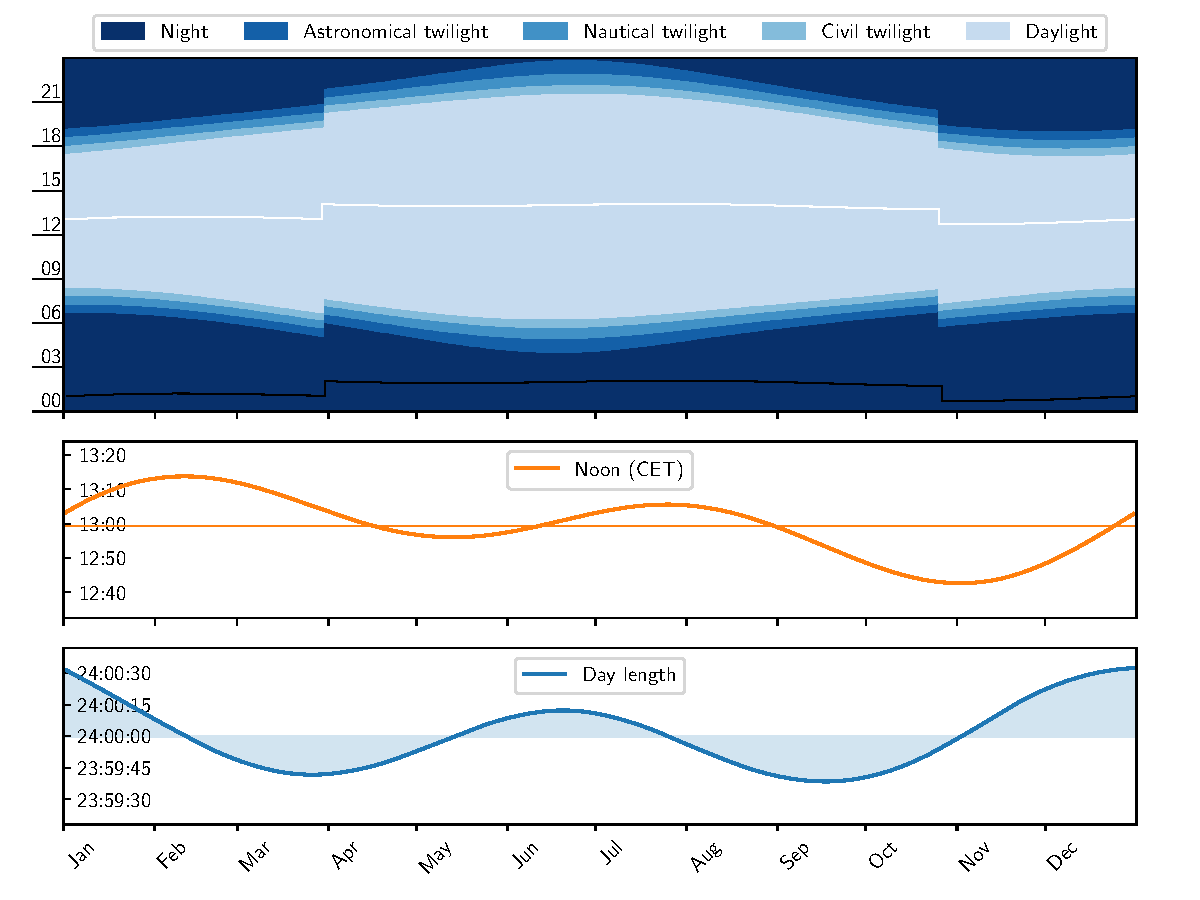
\includegraphics[width=\textwidth]{./sun_graph.pdf}
    \caption{
        Sunrise and sunset times at \textit{Monte Perdido} in local 
        time [data from \texttt{TimeAndDate}].
    }
    \label{fig:sunrise_sunset}
\end{figure}

Then, the natural question is: where is the sun at 12:00 if it is not at its 
highest point? We will answer this question by digging into the math and physics
at play, and discover the beautiful figure drawn by the sun: the analemma.

Someone actually did this experiment and recorded the sun's position
throughout the year 
[\href{https://www.youtube.com/watch?v=Deli5COMJhs}{timelapse link}].


\newpage
The analemma depends on three parameters:
\begin{itemize}
    \item the Earth's axial tilt $\epsilon$;
    \item the eccentricity of the Earth's orbit $e$;
    \item the time shift $\sigma$ between the winter solstice and the perihelion.
\end{itemize}
To understand why, let's proceed step by step, starting without any of these
parameters.

We should also note that latitude and longitude only translate the analemma
to a different position in the sky, but do not change its shape.

For simplicity, let's furthermore suppose that the year is exactly $N=365$ solar 
days of $T_d = 86400=24\times 60\times 60$ seconds. This is obviously inacurate, 
but sufficent to reveal the beauty of the phenomenon at play.

\clearpage
\section{The simplest case}
\begin{figure}
    \centering
    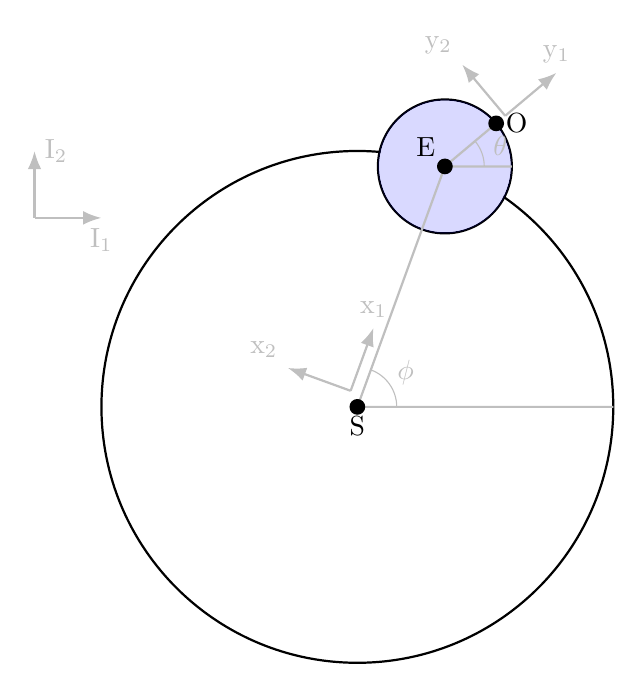
\begin{tikzpicture}
        \pgfmathsetmacro{\rr}{3.25}
        \pgfmathsetmacro{\re}{0.85}
        \pgfmathsetmacro{\ph}{70}
        \pgfmathsetmacro{\th}{40}
        \pgfmathsetmacro{\vv}{0.85}
        \pgfmathsetmacro{\ss}{0.15}
        \pgfmathsetmacro{\bx}{-\rr-\vv}
        \pgfmathsetmacro{\by}{\rr-\vv}
        \coordinate (O) at (0,0);
        \path (O) -- (1,0) coordinate (ex);
        \path (O) -- (0,1) coordinate (ey);
        \path (O) -- (\ph:1) coordinate (u1);
        \path (O) -- ({cos(\ph+90)},{sin(\ph+90)}) coordinate (u2);
        \path (O) -- (\th:1) coordinate (v1);
        \path (O) -- ({cos(\th+90)},{sin(\th+90)}) coordinate (v2);
        \coordinate (A) at (\rr,0);
        \coordinate (E) at ({\rr*cos(\ph)},{\rr*sin(\ph)});
        \coordinate (A0) at ($ (E)!19/20!(O) + \ss*(u2) $);
        \coordinate (A1) at ($ (A0) + \vv*(u1) $);
        \coordinate (A2) at ($ (A0) + \vv*(u2) $);
        \coordinate (S1) at ($ (E) + \re*(ex) $);
        \coordinate (S2) at ($ (E) + \re*(v1) $);
        \coordinate (E0) at ($ (E) + \re*(v1) + \ss*(v1) $);
        \coordinate (E1) at ($ (E0) + \vv*(v1) $);
        \coordinate (E2) at ($ (E0) + \vv*(v2) $);
        \coordinate (B0) at ({\bx}, {\by});
        \coordinate (B1) at ({\bx+\vv}, {\by});
        \coordinate (B2) at ({\bx}, {\by+\vv});
        \draw[thick,-Latex, lightgray] (B0) -- (B1) node[below] {$\mathrm{I}_1$};
        \draw[thick,-Latex, lightgray] (B0) -- (B2) node[right] {$\mathrm{I}_2$};
        \draw[thick,-Latex, lightgray] (A0) -- (A1) node[above] {$\mathrm{x}_1$};
        \draw[thick,-Latex, lightgray] (A0) -- (A2) node[above left] {$\mathrm{x}_2$};
        \draw[thick,-Latex, lightgray] (E0) -- (E1) node[above] {$\mathrm{y}_1$};
        \draw[thick,-Latex, lightgray] (E0) -- (E2) node[above left] {$\mathrm{y}_2$};
        \node at (O) [anchor=north] {S};
        \draw[thick] (O) circle (\rr);
        \draw[thick] (E) circle (\re);
        \fill[color=white] (E) circle (\re*0.98);
        \fill[opacity=0.15, color=Blue] (E) circle (\re);
        \node at (E) [above left] {E};
        \node at (S2) [right] {O};
        \draw[thick,-, lightgray] (S1) -- (E) -- (S2);
        \draw[thick,-, lightgray] (A) -- (O) -- (E);
        \pic [draw, -, "$\theta$", angle eccentricity=1.5, lightgray] {angle = S1--E--S2};
        \pic [draw, -, "$\phi$", angle eccentricity=1.5, lightgray] {angle = A--O--E};
        \fill (O) circle (0.1);
        \fill (S2) circle (0.1);
        \fill (E) circle (0.1);
    \end{tikzpicture}
\end{figure}

The Earth (E) is revolving counterclockwise around the sun (S) in a circular 
orbit of radius $a$, with angular velocity $\dot \phi=\Omega$.
An observer (O) is rotating counterclockwise around the Earth's axis at a 
distance $R$ with angular velocity $\dot \theta=\omega$.

The night sky completes a full rotation to an Earth-based observer in just 
under 24 hours. The extra $\sim 4$ minutes account for the fact that, during 
that time, the Earth also moves slightly along its orbit around the sun - by
about $2\pi/N$ radians. As a result, Earth must rotate a bit more for the 
Sun to return to the same position in the sky.

This period is called the \textit{sidereal day}, noted here $T_s$. 
We experience $N$ solar days in a year, but the Earth actually completes $N+1$ 
sidereal days in the same time.
\begin{align}
    \dot\phi = \Omega = \frac{2\pi}{N T_d} \qquad\qquad
    \dot\theta = \omega = \frac{2\pi}{T_s} = (N+1) \Omega
\end{align}

We want to find the position of the sun at a given time $t$ in the Earth's 
frame:
\begin{equation}
    \begin{aligned}
        \overrightarrow{OS} &= \overrightarrow{OE} + \overrightarrow{ES}\\
        &= -R \mathrm{y}_1 - a \mathrm{x}_1\\
        &= -R \mathrm{y}_1 - a \Big[\cos(\phi-\theta) \mathrm{y}_1 + \sin(\phi-\theta) \mathrm{y}_2\Big].
    \end{aligned}
\end{equation}
Since $R/a \approx 4\times 10^{-5}$, we will neglect the term $R y_1$.
From here on, we will use the direction vector 
$s\approx \overrightarrow{OS}/\|\overrightarrow{OS}\|$ that neglects
the $R$ term. Rewriting $\phi-\theta$, and expressing 12:00 on day $k$ 
as $t_{k}=T_d/2 + kT_d$, we get:
\begin{align}
    s(t) &= -\Big[\cos(2\pi t/T_d) \mathrm{y}_1 + \sin(2\pi t/T_d) \mathrm{y}_2\Big],\\
    s(t_{k}) &= \mathrm{y}_1.
\end{align}

\section{Effect of the Earth's axial tilt}
\begin{figure}
    \centering
    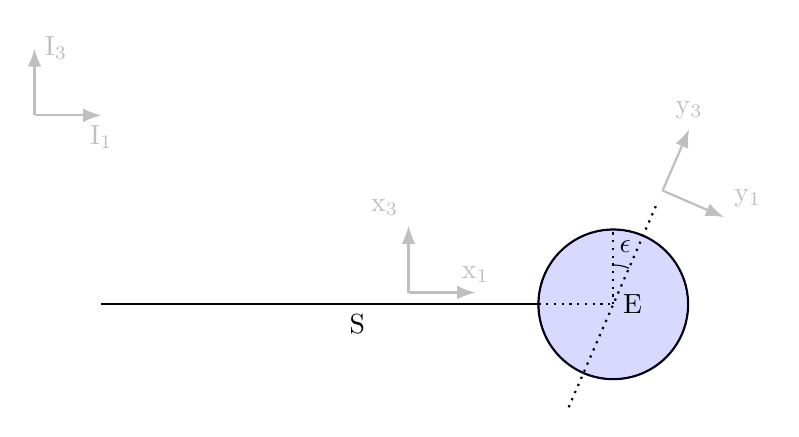
\begin{tikzpicture}
        \pgfmathsetmacro{\rr}{3.25}
        \pgfmathsetmacro{\re}{0.95}
        \pgfmathsetmacro{\ree}{1.5*\re}
        \pgfmathsetmacro{\ph}{70}
        \pgfmathsetmacro{\eps}{23.44}
        \pgfmathsetmacro{\vv}{0.85}
        \pgfmathsetmacro{\ss}{0.15}
        \pgfmathsetmacro{\bx}{-\rr-\vv}
        \pgfmathsetmacro{\by}{\rr-\vv}
        \coordinate (O) at (0,0);
        \path (O) -- (1,0) coordinate (ex);
        \path (O) -- (0,1) coordinate (ey);
        \path (O) -- ({sin(\eps)},{cos(\eps)}) coordinate (u1);
        \path (O) -- ({cos(\eps)},{-sin(\eps)}) coordinate (u2);
        \coordinate (A) at (\rr,0);
        \coordinate (E) at ({\rr},{0});
        \coordinate (A0) at ($ (E)!4/5!(O) + \ss*(ey) $);
        \coordinate (A1) at ($ (A0) + \vv*(ex) $);
        \coordinate (A2) at ($ (A0) + \vv*(ey) $);
        \coordinate (S1) at ($ (E) + \re*(u1) $);
        \coordinate (S2) at ($ (E) + \re*(ey) $);
        \coordinate (E0) at ($ (E) + \ree*(u1) + \ss*(u1) $);
        \coordinate (E1) at ($ (E0) + \vv*(u1) $);
        \coordinate (E2) at ($ (E0) + \vv*(u2) $);
        \coordinate (B0) at ({\bx}, {\by});
        \coordinate (B1) at ({\bx+\vv}, {\by});
        \coordinate (B2) at ({\bx}, {\by+\vv});
        \draw[thick,-Latex, lightgray] (B0) -- (B1) node[below] {$\mathrm{I}_1$};
        \draw[thick,-Latex, lightgray] (B0) -- (B2) node[right] {$\mathrm{I}_3$};
        \draw[thick,-Latex, lightgray] (A0) -- (A1) node[above] {$\mathrm{x}_1$};
        \draw[thick,-Latex, lightgray] (A0) -- (A2) node[above left] {$\mathrm{x}_3$};
        \draw[thick,-Latex, lightgray] (E0) -- (E1) node[above] {$\mathrm{y}_3$};
        \draw[thick,-Latex, lightgray] (E0) -- (E2) node[above right] {$\mathrm{y}_1$};
        \node at (O) [anchor=north] {S};
        \draw[thick] (-\rr, 0) -- (O) -- (E);
        \draw[thick] (E) circle (\re);
        \fill[color=white] (E) circle (\re*0.98);
        \fill[opacity=0.15, color=Blue] (E) circle (\re);
        \node at (E) [right] {E};
        % \node at (S2) [right] {O};
        \draw[thick, dotted] (\rr-\re,0) -- (E);
        \draw[thick, dotted] (E) -- ($ (E) +\re*(ey)$);
        \draw[thick, dotted] ($ (E) -\ree*(u1)$) -- ($ (E) +\ree*(u1)$);
        \pic [draw, -, "$\epsilon$", angle eccentricity=1.5] {angle = S1--E--S2};
        % \draw[thick,-, lightgray] (S1) -- (E) -- (S2);
        % \draw[thick,-, lightgray] (A) -- (O) -- (E);
        % \pic [draw, -, "$\phi$", angle eccentricity=1.5, lightgray] {angle = A--O--E};
        % \fill (O) circle (0.1);
        % \fill (S2) circle (0.1);
        % \fill (E) circle (0.1);
    \end{tikzpicture}
\end{figure}

The Earth's axis is tilted by an angle $\epsilon=23.44^\circ$ with respect to
the ecliptic plane. The basis $[\mathrm{y}]$ attached to the Earth's frame is 
now obtained after two rotations: first by $\epsilon$ around the $\mathrm{I}_2$ 
axis, then by $\theta$ around the third axis:
\begin{equation}
    \begin{aligned}[c]
        [ \mathrm{y} ] &= R_3(\theta) R_2(\epsilon) [\mathrm{I}] \\
        [ \mathrm{x} ] &= R_3(\phi) R_2(-\epsilon) R_3(-\theta)[\mathrm{y}].
    \end{aligned}
\end{equation}

The sun's position in the Earth's frame $[\mathrm{y}]$ is now given by:
\begin{equation}
    s = -\mathrm{x}_1 =
    \begin{bmatrix}
        -\cos(\phi)\cos(\epsilon)\cos(\theta) - \sin(\phi)\sin(\theta)\\
        \phantom{+}\cos(\phi)\cos(\epsilon)\sin(\theta)-\sin(\phi) \cos(\theta)\\
        -\cos(\phi)\sin(\epsilon)\phantom{\sin(\theta)+\sin(\phi) \cos(\theta)}
    \end{bmatrix}.
    \label{eq:position}
\end{equation}

\textbf{Where is the sun at 12:00?}

Once again, we insert $t_{k}=kT_d+T_d/2$ for $k=0,1,2,\ldots N-1$ in $s$ to 
derive the sun's position at noon. First let's express the angles $\phi$ and 
$\theta$ in terms of $k$:
\begin{equation}
    \left\{
    \begin{aligned}
        \phi &= \Omega t_{k} = 2\pi \frac{1}{N} (k+\tfrac{1}{2})\\
        \theta &= \omega t_{k} = 2\pi \frac{N+1}{N} (k+\tfrac{1}{2})
    \end{aligned}
    \right\} \implies
    \left\{
    \begin{aligned}
        \phi-\theta &= -N\phi = -2\pi (k+\tfrac{1}{2})\\
        \phi+\theta &= (N+2)\phi = 2\pi k + \pi + 2\cdot 2\pi \frac{k+\tfrac{1}{2}}{N}
    \end{aligned}
    \right\}.
\end{equation}

Using trigonometric identities, we find
\begin{equation}
    \begin{aligned}
        \cos(\phi)\cos(\theta)\vert_{12:00} &= -\cos^2\left(2\pi \frac{k+1/2}{N}\right)\\
        \sin(\phi)\sin(\theta)\vert_{12:00} &= -\sin^2\left(2\pi \frac{k+1/2}{N}\right)\\
        \cos(\phi)\sin(\theta)\vert_{12:00} &= -\frac{1}{2} \sin(2\cdot 2\pi \frac{k+1/2}{N})
        = \sin(\phi)\cos(\theta)\vert_{12:00}.
    \end{aligned}
\end{equation}

With these, we can express the analemma as a 
parametric curve with parameter 
$\beta \in [0,2\pi]$:
\begin{equation}
    s\vert_{12:00}(\beta) =
    \frac{1}{2}
    \begin{bmatrix}
        1+\cos\epsilon\\
        0\\
        0
    \end{bmatrix}+
    \frac{1}{2}
    \begin{bmatrix}
        - (1-\cos\epsilon) \cos(2\beta)\\
        \phantom{+} (1-\cos\epsilon) \sin(2\beta)\\
        \quad\;-2\sin(\epsilon) \cos(\phantom{2}\beta)
    \end{bmatrix}.
    % \begin{bmatrix}
    %     \cos(\epsilon)\cos^2(\beta) + \sin^2(\beta)\\
    %     \tfrac{1}{2}(1-\cos(\epsilon)) \sin(2\beta)\\
    %     -\sin(\epsilon) \cos(\beta)
    % \end{bmatrix}.
\end{equation}

This curve is shown in figure \ref{fig:analemma_easy} for various 
tilt angles $\epsilon$, in the observer's frame, that is, without the 
$\mathrm{y}_1$ component. We can note that beyond $\epsilon=90^\circ$, we
enter in a strange territory where the sun is below the horizon at 12:00, with
the day/night cycle reversed.
\begin{figure}[ht]
    \centering
    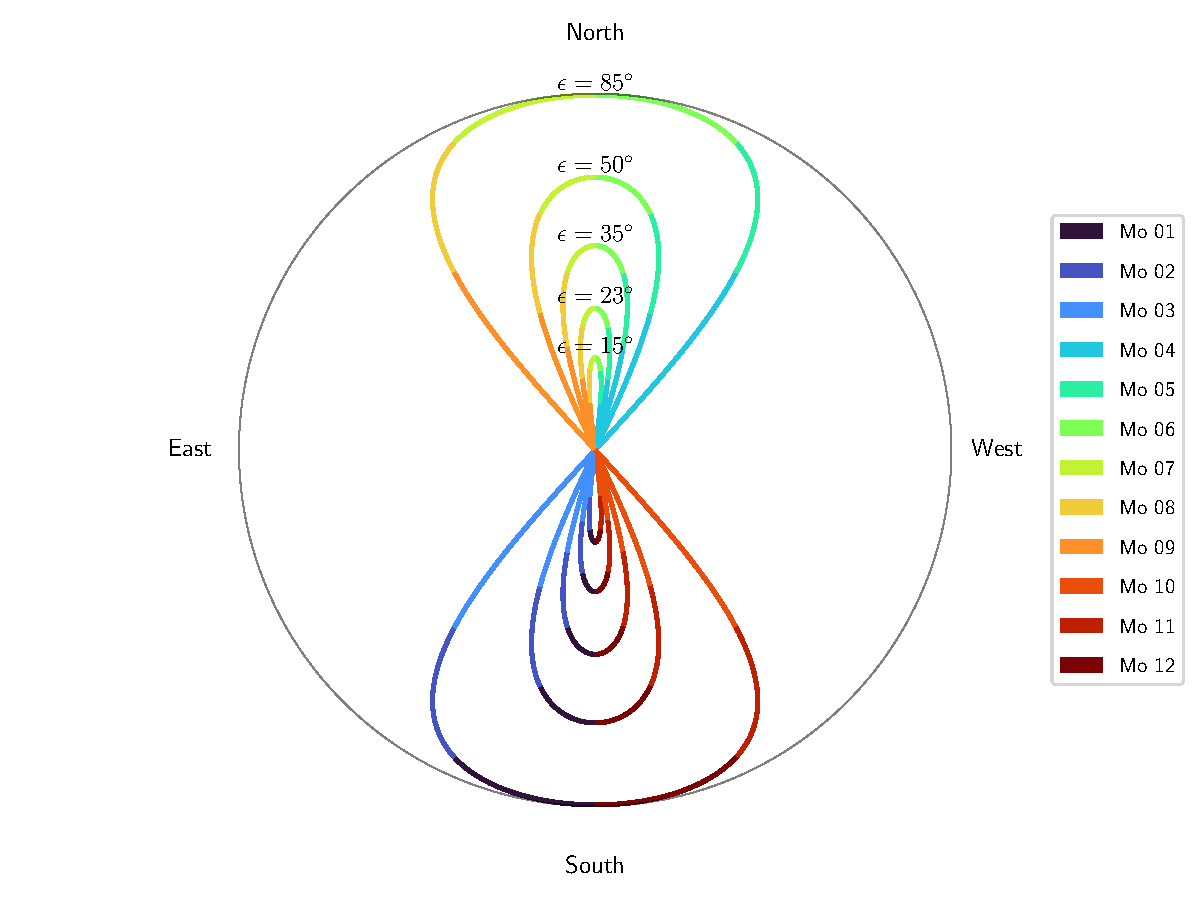
\includegraphics[width=\textwidth]{./analemma_plot.pdf}
    \caption{
        The analemma of 12:00, viewed from the ground at 00°N. 
        The border of the figure is the horizon of the observer. 
        Each month has been assigned a specific color.
    }
    \label{fig:analemma_easy}
\end{figure}


\textbf{When is the sun at its highest point?}

At "solar" noon and midnight, the vector $\mathrm{x}_1$ has no $\mathrm{y}_2$ component:
:
\begin{equation}
    \begin{aligned}
        \cos(\Omega t)\sin\big((N+1)\Omega t\big) \cos(\epsilon) &= \sin(\Omega t) \cos\big((N+1)\Omega t\big)\\
        \iff \quad \sin(N\Omega t)(1-c \cos^2(\Omega t)) &= \frac{c}{2} \cos(N\Omega t) \sin(2\Omega t)
    \end{aligned}
\end{equation}
where $c=1-\cos(\epsilon)$. This equation has no closed form solution for $t^*$,
but we can approximate it around 12:00 with $t^*=kT_d+T_d/2+\delta$, $k=0,1,2\ldots N-1$
:
\begin{equation}
    \left\{
        \begin{aligned}
            \sin(N\Omega t^*) &= -\sin(2\pi\delta / T_d)\\
            \cos(N\Omega t^*) &= -\cos(2\pi\delta / T_d)\\
            \sin(2\Omega t^*) &\approx \sin\big(\tfrac{2\pi}{N} (1+2k)\big)\\
            \cos(\Omega t^*) &\approx \cos\big(\tfrac{\:\pi\:}{N} (1+2k)\big)\\
        \end{aligned}
    \right\} \; \implies \;
    \frac{2\pi \delta}{T_d} \approx \tan(\frac{2\pi \delta}{T_d}) = 
    \frac{c}{2} \frac{\sin(2\cdot 2\pi \tfrac{k+0.5}{N})}{1-c \cos^2(2\pi \tfrac{k+0.5}{N})}.
    \label{eq:noon_shift}
\end{equation}
Noon is off by $\delta$ seconds from the mean solar time, and this shift
oscillates twice a year as we can see with the factor at the numerator of 
\eqref{eq:noon_shift} and in figure \ref{fig:noon_shift}. 
The approximation can be simplified with $\tan(x) \approx x$ 
("approx. 2") and even further by removing the denominator ("approx. 3"),
providing acceptable results until quite large tilt angles $\epsilon$.

\begin{figure}[ht]
    \centering
    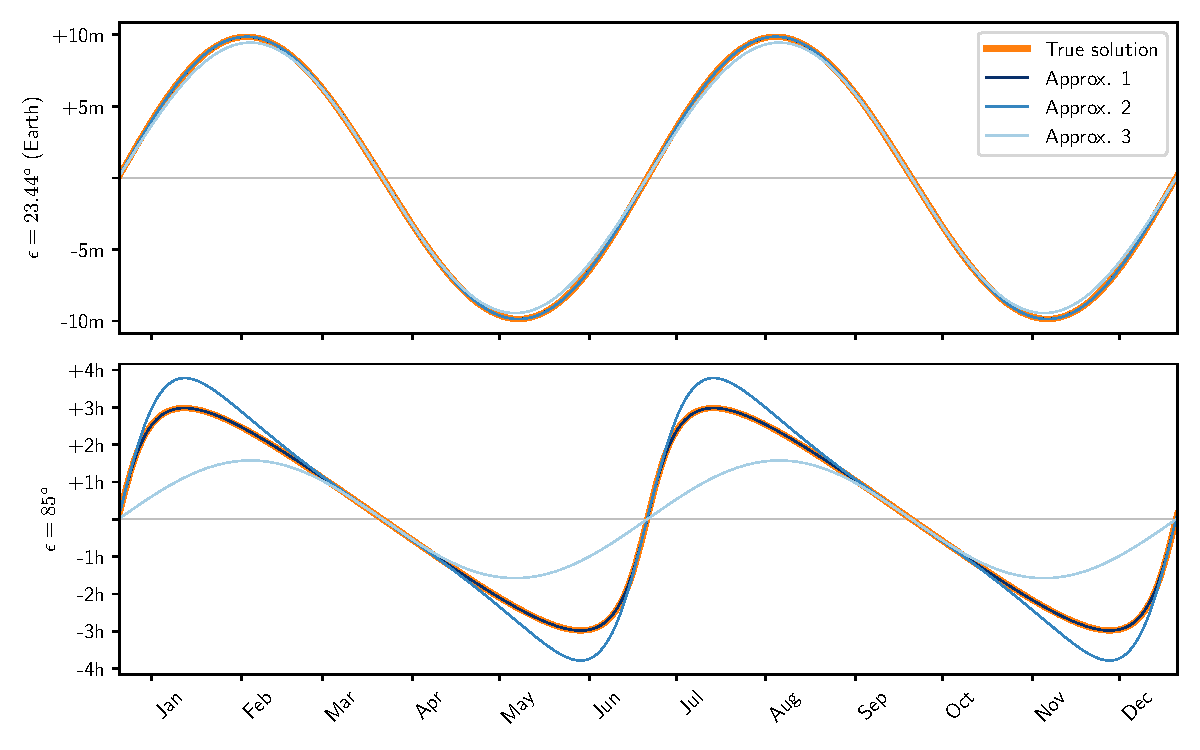
\includegraphics[width=\textwidth]{./noon_computed.pdf}
    \caption{
        Apparent noon time throughout the year for two different axial tilt angles $\epsilon$.
    }
    \label{fig:noon_shift}
\end{figure}

\textbf{An intuitive explanation}

If we consider the Earth's rotating frame,
the sun is revolving around the earth, but also moving up 
(winter and spring) and down (autumn and summer) its equatorial plane.

This vertical motion has a period of one year: the sun reaches its highest point
at the summer solstice, and its lowest point at the winter solstice, for people 
in the northern hemisphere. Since the sun's total motion is constant in this 
cicular orbit model, its horizontal motion must slow down when the vertical 
motion is at its highest \textit{in absolute value}. 

The sun's eastward velocity is thus at its highest
at both solstices, and at its lowest at both equinoxes, producing a
motion of period half a year. The sun's horizontal position is simply the
integral of this velocity as we can see in figure 
\ref{fig:noon_shift}.

\clearpage
\section{Effect of Earth's orbit eccentricity}

\begin{figure}
    \centering
    \begin{tikzpicture}
        \pgfmathsetmacro{\ra}{3.75}
        \pgfmathsetmacro{\rb}{2.5}
        \pgfmathsetmacro{\re}{0.85}
        \pgfmathsetmacro{\nnu}{55}
        \pgfmathsetmacro{\gam}{20}
        \pgfmathsetmacro{\vv}{0.85}
        \pgfmathsetmacro{\ss}{0.15}
        \pgfmathsetmacro{\bx}{-\ra-2*\vv}
        \pgfmathsetmacro{\by}{\ra-\vv}
        \pgfmathsetmacro{\c}{sqrt(\ra*\ra-\rb*\rb)}
        \pgfmathsetmacro{\e}{\c/\ra}
        \pgfmathsetmacro{\dd}{0.07}
        \pgfmathsetmacro{\cosn}{(cos(\nnu)-\e)/(1-\e*cos(\nnu))}
        \pgfmathsetmacro{\sinn}{(sqrt(1-\e*\e)*sin(\nnu))/(1-\e*cos(\nnu))}
        \pgfmathsetmacro{\mm}{\nnu-\e*sin(\nnu)*180/pi}
        \coordinate (C) at (0,0);
        \coordinate (S) at (\c,0);
        \path (C) -- (1, 0) coordinate (e1);
        \path (C) -- (0, 1) coordinate (e2);
        \path (C) -- ({cos(\gam)},{-sin(\gam)}) coordinate (i1);
        \path (C) -- ({sin(\gam)},{cos(\gam)}) coordinate (i2);
        \path (C) -- ({\cosn},{\sinn}) coordinate (u1);
        \path (C) -- ({-\sinn},{\cosn}) coordinate (u2);
        \coordinate (A) at (\ra,0);
        \coordinate (E) at ({\ra*cos(\nnu)},{\rb*sin(\nnu)});
        \coordinate (EH) at ({\ra*cos(\nnu)},{0});
        \coordinate (EC) at ({\ra*cos(\nnu)},{\ra*sin(\nnu)});
        \coordinate (EM) at ({\ra*cos(\mm)},{\ra*sin(\mm)});
        \coordinate (A0) at ($ (E)!19/20!(S) + \ss*(u2) $);
        \coordinate (A1) at ($ (A0) + \vv*(u1) $);
        \coordinate (A2) at ($ (A0) + \vv*(u2) $);
        \coordinate (B0) at ({\bx}, {\by});
        \coordinate (B1) at ($ (B0) + \vv*(i1) $);
        \coordinate (B2) at ($ (B0) + \vv*(i2) $);
        \coordinate (BH) at ($ (B0) + 2*\vv*(e1) $);
        \fill[blue, opacity=0.1] (S) -- (A) arc(0:\nnu:\ra);
        \fill[orange, opacity=0.1] (O) -- (A) arc(0:\mm:\ra);
        \node at (A) [anchor=west] {A};
        \node at (C) [anchor=north] {O};
        \node at (S) [anchor=north] {S};
        \draw[thick] (C) ellipse ({\ra} and {\rb});
        \draw[thick, lightgray, dotted] (C) circle ({\ra});
        \draw[thick, lightgray, dotted] (EH) -- (EC);
        \node at (E) [above right] {P};
        \node at (EM) [anchor=west] {P''};
        \node at (EC) [above right] {P'};
        \node at (EH) [anchor=north] {D};
        \draw[thick, dotted, lightgray] (S) -- (C) -- (EC);
        \draw[thick, -, lightgray] (A) -- (S) -- (E) node[pos=0.6, right] {$r$};
        \pic [draw, -, "$\nu$", angle eccentricity=1.5, lightgray] {angle = A--S--E};
        \pic [draw, -, "$E$", angle eccentricity=1.4, lightgray] {angle = A--O--EC};
        \pic [draw, -, "$M$", angle radius=30, angle eccentricity=1.2, lightgray] {angle = A--O--EM};
        \pic [draw, -, "$\gamma$", angle radius=40, angle eccentricity=1.2, lightgray] {angle = B1--B0--BH};
        \fill (A) circle (\dd);
        \fill (C) circle (\dd);
        \fill (S) circle (\dd);
        \fill (E) circle (\dd);
        \fill (EH) circle (\dd);
        \fill (EM) circle (\dd);
        \fill (EC) circle (\dd);
        \draw[thick, dashed, lightgray] (B0) -- (BH);
        \draw[thick,-Latex, lightgray] (B0) -- (B1) node[below] {$\mathrm{I}_1$};
        \draw[thick,-Latex, lightgray] (B0) -- (B2) node[right] {$\mathrm{I}_2$};
        \draw[thick,-Latex, lightgray] (A0) -- (A1) node[left=-3pt] {$\mathrm{x}_1$};
        \draw[thick,-Latex, lightgray] (A0) -- (A2) node[below] {$\mathrm{x}_2$};
    \end{tikzpicture}
\end{figure}

The Earth's orbit is not a perfect circle, but an ellipse with semi-major axis
$a$ and semi-minor axis $b$. For the earth, the orbit eccentricity 
$e=\sqrt{1-b^2/a^2}\approx 0.017$ is relatively small, but enough to have a
noticeable effect on the analemma. The eccentricity $e\approx 0.75$ in the 
figure above is exaggerated for clarity.

In the early 17th century, Johannes Kepler stated his famous \textit{laws of
planetary motion}:
\begin{enumerate}
    \item The orbit of a planet is an ellipse with the sun at one focus.
    \item A line segment joining a planet and the sun sweeps out equal areas during
        equal intervals of time.
    \item The square of the orbital period of a planet is proportional to the cube
        of the semi-major axis of its orbit.
\end{enumerate}

\textbf{Anomalies}

To describe efficiently a planet's position along its elliptical orbit at a 
given time, astronomers use three angular parameters called \textit{anomalies} to 
stress the difference with a circular orbit. 

\begin{enumerate}
    \item \textit{True anomaly} $\nu$, the angle between the direction of 
    perihelion and the Earth.
    \item \textit{Eccentric anomaly} $E$, an  auxiliary  angle  used to simplify
    calculations.
    \item \textit{Mean anomaly} $M=\Omega t$, increasing linearly with time.
\end{enumerate}

While $M(t)$ increases linearly, Kepler's second law implies that $\nu(t)$ does not.
Because the Earth moves faster near perihelion and slower near aphelion, 
the apparent motion of the Sun in the sky varies over the year.

Kepler's second law states that the blue and orange areas in the figure above 
are equal:
\begin{align}
    |AOP''| &= |ASP'| = |AOP'| - |OSP'|\\
    \frac{a^2 M}{2} &= \frac{a^2 E}{2} - \frac{(ae) (a\sin e)}{2}\\
    M &= E - e \sin E \label{eq:keplereq}.
\end{align}
The resulting equation is known as \textit{Kepler's equation} and has no closed 
form solution for $E$ in terms of $M$. Once the eccentric anomaly $E$ has been 
derived from the mean anomaly $M$, it remains to find the true anomaly $\nu$:
\begin{align}
    r &= a(1-e \cos E) \label{eq:r}\\[6pt]
    \cos \nu &= \frac{\cos E - e}{1 - e \cos E}, \label{eq:cosnu}\\[0pt]
    \sin \nu &= \frac{\sqrt{1-e^2} \sin E}{1-e\cos E}, \label{eq:sinnu}\\
    r &= a\: \frac{1-e^2}{1+e \cos \nu}
\end{align}

The relationships \eqref{eq:r}, \eqref{eq:cosnu} and \eqref{eq:sinnu} 
were respectively derived by:
\begin{gather}
    \begin{aligned}
        r^2 &= \|SD\|^2+ \|DP\|^2 = b^2 \sin^2 E + (ae - a \cos E)^2\\
        &= a^2 \left[(1-e^2) (1-\cos^2 E) + (e^2 - 2e \cos E + \cos^2 E)\right]\\
        &= a^2 \left[ 1 - 2e \cos E + e^2 \cos^2 E\right] = a^2 (1-e \cos E)^2
    \end{aligned}\\[12pt]
    \begin{aligned}
        \|OD\| + \|DS\| &= \|OS\|\\
        a \cos E - r \cos \nu &= ae\\
        a \cos E - a (1-e \cos E) \cos \nu &= ae
        % \implies \cos \nu &= \frac{\cos E - e}{1-e \cos E}
    \end{aligned}\\[12pt]
    \begin{aligned}
        \|DP\| = r \sin \nu &= b \sin E\\
        a(1-e\cos E) \sin \nu &= a\sqrt{1-e^2} \sin E
    \end{aligned}
\end{gather}

The true anomaly can be approximated from the mean anomaly
via a Fourier expansion:
\begin{equation}
    \nu = M + (2e - \tfrac{1}{4}e^3)\sin(M) + \tfrac{5}{4}e^2 \sin(2M) + 
    \tfrac{13}{12}e^3 \sin(3M) + \mathcal{O}(e^4).
\end{equation}

Perihelion ($\nu=0$) and winter solstice ($\phi=0$) do not have to coincide,
even though they are quite close currently for Earth which gets closest to the 
sun in early january. Introducing the angle $\gamma=\Omega\sigma$ between the 
winter solstice and perihelion, we can relate the orbital position $\phi$ and 
its first order approximation directly to time:
\begin{equation}
    \begin{aligned}
        \mu &= M + \gamma = \Omega t\\
        \phi &= \nu + \gamma = \mu + \underbrace{2e \sin(\mu-\gamma)}_{\phi_1} + \mathcal{O}(e^2)
    \end{aligned}
\end{equation}

\textbf{Where is the sun at 12:00?}

We want an approximation of the sun's position, given by equation 
\eqref{eq:position}, at noon, by taking into account the
Earth's orbit eccentricity with our new estimate $\phi(t)$.

Using the first order approximation only as it is
sufficiently painful already, we expand $\cos\phi$, 
$\sin\phi$ and $r$ in terms of $\mu$ and $\gamma$:
\begin{equation}
    \begin{aligned}
        \cos \phi &= \cos \mu \cos\phi_1 - \Sin \mu \sin\phi_1 = 
            \cos\mu -e\cos\gamma(1-\cos2\mu) + e\Sin\gamma\Sin2\mu + \mathcal{O}(e^2)\\
        \sin \phi &= \Sin \mu \cos\phi_1 + \cos \mu \sin\phi_1 = 
            \Sin\mu -e\Sin\gamma(1+\cos2\mu) + e\cos\gamma\Sin2\mu + \mathcal{O}(e^2)\\
        r/a &= \tfrac{1-e^2}{1+e\cos(\phi-\gamma)} 
            = 1 - e\cos(\mu-\gamma) + \mathcal{O}(e^2) 
            % = 1 - e (\cos\gamma \cos\mu - \Sin\gamma \sin\mu) + \mathcal{O}(e^2) 
    \end{aligned}
\end{equation}

Let's first recall the expressions for noon, the Earth's angular position 
$\theta$, and let's derive a useful relation for integer multiples of the 
angular position $\mu$:
\begin{align}
    t_k &= k T_d + \tfrac{T_d}{2}\\
    \mu_k &= \Omega t_k = 2\pi \tfrac{k+1/2}{N}\\
    \theta &= (N+1)\Omega t = (N+1)\mu\\
    (N+\ell)\Omega t_{k} &= 2\pi k + \pi + \ell \mu_k
\end{align}

Playing around with the trigonometric product-to-sum identities, we find:
\begin{align}
    \cos (\phi_k) \cos (\theta_k) &\approx \tfrac{-1}{2} (1+\cos2\mu) 
        + \tfrac{e}{2} \cos\gamma( \cos\mu - \cos3\mu) 
        - \tfrac{e}{2} \Sin\gamma( \Sin\mu + \Sin3\mu),
        \label{eq:coscos}\\[3pt]
    \Sin (\phi_k) \Sin (\theta_k) &\approx \tfrac{-1}{2} (1-\cos2\mu) 
        - \tfrac{e}{2} \cos\gamma (\cos\mu - \cos3\mu)
        + \tfrac{e}{2} \Sin\gamma (\Sin\mu + \Sin3\mu),
        \label{eq:sinsin}\\[3pt]
    \cos (\phi_k) \Sin (\theta_k) &\approx -\tfrac{1}{2} \sin(2\mu) 
        + \tfrac{e}{2} \cos\gamma (3\Sin\mu - \Sin3\mu)
        - \tfrac{e}{2} \Sin\gamma (\phantom{3}\cos\mu - \cos3\mu),
        \label{eq:cossin}\\[3pt]
    \Sin (\phi_k) \cos (\theta_k) &\approx -\tfrac{1}{2} \sin(2\mu) 
        - \tfrac{e}{2} \cos\gamma (\phantom{3}\Sin\mu + \Sin3\mu)
        + \tfrac{e}{2} \Sin\gamma (3\cos\mu + \cos3\mu).
        \label{eq:sincos}
\end{align}

With the elliptical orbit, the position of the sun in the Earth's frame, 
obtained previously in equation \eqref{eq:position} must now be scaled by 
the varying distance $r$:
\begin{equation}
    s = -\frac{r}{a} \mathrm{x}_1 =
    -\frac{r}{a}\begin{bmatrix}
        -\cos(\phi)\cos(\epsilon)\cos(\theta) - \sin(\phi)\sin(\theta)\\
        \phantom{+}\cos(\phi)\cos(\epsilon)\sin(\theta)-\sin(\phi) \cos(\theta)\\
        -\cos(\phi)\sin(\epsilon)\phantom{\sin(\theta)+\sin(\phi) \cos(\theta)}
    \end{bmatrix}+\mathcal{O}(e^2).
    \label{eq:positionEllipse}
\end{equation}

Inserting the approximations \eqref{eq:coscos}--\eqref{eq:sincos} into
equation \eqref{eq:positionEllipse} allows us to approximate the analemma 
up to first order in $e$ with a curve parametrized by $\mu \in [0,2\pi]$:
\begin{align}
    s\vert_{12:00}(\mu) &=
    \begin{bmatrix}
        \frac{1+\cos\epsilon}{2}-\frac{1-\cos\epsilon}{2} \cos2\mu
            -\phantom{2}e(\cos\epsilon\cos\gamma\cos\mu + \Sin\gamma\Sin\mu) 
            + \delta_1\\[6pt]
        \phantom{\frac{1+\cos\epsilon}{2}-{}}\frac{1-\cos\epsilon}{2} \Sin2\mu
            + 2e (\cos\epsilon\cos\gamma \Sin\mu - \Sin\gamma \cos\mu) 
            + \delta_2\\[6pt]
        -\Sin\epsilon \cos\mu + e\:\tfrac{\sin\epsilon}{2}(
            3\cos\gamma-\cos\gamma\cos2\mu-\Sin\gamma\Sin2\mu
        )
        % \phantom{{}+ \tfrac{5}{2}e\cos\epsilon\Sin\beta} \\[3pt]
        % \phantom{(1+\cos\epsilon)+{}}(1-\cos\epsilon) \big(\Sin2\beta + e\Sin\beta + e\Sin3\beta \big) + \textcolor{Red}{\tfrac{5}{2}e\cos\epsilon\Sin\beta}\\[3pt]
        % \quad\;-2\Sin\epsilon \cos\beta
    \end{bmatrix}
    +\mathcal{O}(e^2)\\[9pt]
    \begin{bmatrix}
        \delta_1\\
        \delta_2
    \end{bmatrix} &=
    e\:\tfrac{1-\cos\epsilon}{4}
    \begin{bmatrix}
        \cos\gamma & -\Sin\gamma\\
        \Sin\gamma & \phantom{-}\cos\gamma
    \end{bmatrix}
    \begin{bmatrix}
        \cos\mu - \cos3\mu\\
        \Sin\mu + \Sin3\mu
    \end{bmatrix}%\\
    % \delta_1 &= e\:\tfrac{1-\cos\epsilon}{4}\big(
    %     \cos\gamma(\cos\mu-\cos3\mu)-\Sin\gamma(\Sin\mu+\Sin3\mu)
    % \big) \\[3pt]
    % \delta_2 &= e\:\tfrac{1-\cos\epsilon}{4}\big(
    %     \cos\gamma(\Sin\mu+\Sin3\mu)+\Sin\gamma(\cos\mu-\cos3\mu)
    % \big)
\end{align}

Quite an expression! The extra terms $\delta_1$ and $\delta_2$ were put aside
because they only slightly contribute to the overall shape of the analemma.
Let's now consider the case $\gamma=0$ to measure the effect of the
Earth's orbit eccentricity without the complication of the perihelion shift.

In that case, the main effect of the Earth's orbit eccentricity is to break 
the vertical symmetry of the analemma. 
In the second component of $s$, the term $2e\cos\epsilon\Sin\mu$
tends to push the analemma towards the left during the first half of the year
and towards the right during the second half. As a consequence, the analemma's
lower loop of winter solstice gets widened, while the upper loop of summer 
solstice gets narrowed.

The effect would be exactly the opposite if we had $\gamma=\pi$,
that is, if the perihelion was at the summer solstice. 
On the other hand, small angles $\gamma$ tend to rotate the analemma, 
breaking the vertical symmetry. The situation with arbitrary angles $\gamma$
is however quite intricate, and should just be enjoyed visually.

% The main effect of the Earth's orbit eccentricity is to break the vertical
% symmetry of the analemma. The term highlighted in red tends to widen the analemma
% around the winter solstice ($\beta\in[-\pi/2,\pi/2]$), and narrow it around the summer solstice.



\end{document}